%\newcommand{\ein}[2]{(#1) (#2 Punkte)}


\begin{Large}
\textbf{Teil I: Offene Aufgaben (40 Punkte)}
\end{Large}
\\
\\
\\
\textbf{Allgemeine Anweisungen für offene Fragen:}
\\
\renewcommand{\labelenumi}{(\roman{enumi})}
\begin{enumerate}
\item
Ihre Antworten müssen alle Rechenschritte enthalten,
diese müssen klar ersichtlich sein.
Verwendung korrekter mathematischer Notation wird erwartet
und fliesst in die Bewertung ein.

\item
Ihre Antworten zu den jeweiligen Teilaufgaben müssen in den dafür vorgesehenen Platz geschrie-
ben werden. Sollte dieser Platz nicht ausreichen, setzen Sie Ihre Antwort auf der Rückseite oder
dem separat zur Verfügung gestellten Papier fort. Verweisen Sie in solchen Fällen ausdrücklich
auf Ihre Fortsetzung. Bitte schreiben Sie zudem Ihren Vor- und Nachnamen auf jeden separaten
Lösungsbogen.

\item
Es werden nur Antworten im dafür vorgesehenen Platz bewertet. Antworten auf der Rückseite
oder separatem Papier werden nur bei einem vorhandenen und klaren Verweis darauf bewertet.

\item
Die Teilaufgaben werden mit den jeweils oben auf der Seite angegebenen Punkten bewertet.

\item
Ihre endgültige Lösung jeder Teilaufgabe darf nur eine einzige Version enthalten.

\item
Zwischenrechnungen und Notizen müssen auf einem getrennten Blatt gemacht werden. Diese
Blätter müssen, deutlich als Entwurf gekennzeichnet, ebenfalls abgegeben werden.
\end{enumerate}

\newpage
\section*{\hfil Aufgaben \hfil}
\vspace{1cm}
\section*{Aufgabe 1 (40 Punkte)}
\vspace{0.4cm}
\subsection*{\aufgabe{a}{10}}
Ein Monopolist stellt zwei Güter her.
In Abhängigkeit von den Preisen $ p_1 $ und $ p_2 $ je Mengeneinheit von Gut $ 1 $ bzw. Gut $ 2 $ lautet die
\begin{align*}
	&\textrm{Absatzmenge für Gut $ 1 $:} \quad 
	x = 30 - 3 p_1 + 2 p_2\\
	&\textrm{Absatzmenge für Gut $ 2 $:} \quad
	y = 20 + p_1 - p_2.
\end{align*}
\begin{enumerate}
	\item[\textbf{(a1)}]
	Stellen Sie den Gesamtumsatz $ U(x,y) $ nur durch $ x $ und $ y  $ dar.
	\item[\textbf{(a2)}] 
	Die Produktionskosten lauten
	\begin{align*}
		K(x,y) = x^2 + xy + y^2.
	\end{align*}
	Bei welchen Produktionsmengen $ x^\ast  $ und $ y^\ast $ wird der Reingewinn $ G(x,y) $ maximal?\\
	Wie gross ist der maximale Reingewinn?
\end{enumerate}
\ \\
\subsection*{\aufgabe{b}{14}}
Je nach Konjunktur (gut, mittel, schlecht) haben drei Aktien unterschiedliche zu erwartende Auszahlungen.
\begin{table}[H]
	\centering
	%
	\begin{tabular}{|l |c |c |c|}
		\hline
		\multirow{3}{*}{Konjunktur}
		& erwartete Auszahlung	& erwartete Auszahlung & erwartete Auszahlung\\
		& pro Einheit von & pro Einheit von & pro Einheit von\\
		& Aktie 1 & Aktie 2	& Aktie 3\\
		\hline
		gut & $ 2 $  &  $ a $ &  $ 5 $ \\ 
		\hline
		mittel & $ 1 $ & $ 1 $ & $ 1 $  \\ 
		\hline
		schlecht & $ 0 $ & $ 1 $ & $ a $ \\
		\hline
	\end{tabular}%
\end{table}
Gesucht sind geeignete Kombinationen dieser Geldanlagen (Käufe, respektive Leerverkäufe), die bei guter Konjunktur die Auszahlung $ 7'000 $, bei mittlerer Konjunktur die Auszahlung $ 5'000 $ und bei schlechter Konjunktur die Auszahlung $ 1'000 $ ergeben.
\begin{enumerate}
	\item[\textbf{(b1)}]
	Bestimmen Sie ein lineares Gleichungssysteme für die benötigten Einheiten $ x_i \in \mathbb{R} $ der Anteile an Aktie $ i \in \{1,2,3\} $, die man haben muss, um bei jeder Konjunkturlage die gewünschte Auszahlung erreichen zu können.
	\item[\textbf{(b2)}] 
	Für welche Werte von $ a \in \mathbb{R} $ gibt es eine eindeutige Kombination?
	Für welche Werte von $ a \in \mathbb{R} $ gibt es keine mögliche Kombination?
	Für welche Werte von $ a \in \mathbb{R} $ gibt es unendlich viele mögliche Kombinationen?
	\item[\textbf{(b3)}]
	Berechnen Sie im Falle einer eindeutigen Lösung die Lösung $ (x_1,x_2,x_3) $ (in Abhängigkeit von $ a $).
	\item[\textbf{(b4)}]
	Beschreiben Sie die Lösungsgesamtkeit der möglichen Kombinationen, wenn es unendlich viele Lösungen gibt.
\end{enumerate}

\ \\
\subsection*{\aufgabe{c}{10}}
Für einen elliptischen Tisch mit den Halbachsen $ a > 0  $ und $ b > 0 $ ist eine flächenmässig möglichst grosse rechteckige Auflage anzufertigen, die an keiner Stelle übersteht.
\begin{enumerate}
	\item[\textbf{(c1)}]
Welche Ausmasse (Länge und Breite) hat die rechteckige Auflage?
\item[\textbf{(c2)}]
Wie gross ist die maximale Fläche?
\end{enumerate}
\textit{Wichtige Bemerkung}: Eine Abklärung, ob es sich wirklich um ein Maximum handelt, wird \textbf{nicht} verlangt, weil es offensichtlich ein Maximum geben muss.
\ \\
\subsection*{\aufgabe{d}{6}}
\begin{enumerate}
	\item[\textbf{(d1)}]
	Gesucht sind alle (positiven) Funktionen $ f(x) $, welche für alle $ x > 0 $ die Elastizität
	\begin{align*}
		\varepsilon_f(x) = \frac{1}{x}
	\end{align*}
	besitzen.\\
	\textit{Tipp:} Erinnern Sie sich, dass für positive Funktonen $ f(x) $ gilt:
	\begin{align*}
		\frac{d}{dx} \ln(f(x)) = \rho_f(x) 
		\ \textrm{und} \
		\varepsilon_f(x) = x \cdot \rho_f(x),
	\end{align*}
	wobei $ \rho_f $ die Wachstumsrate von $ f $ ist.
	\item[\textbf{(d2)}]
	Welche positive Funktion $ f(x) $ mit $ f(1) = 1 $ besitzt die Elastizität $ \varepsilon_f(x) = \frac{1}{x} $ für alle alle $ x >0 $.
\end{enumerate}
\newpage


\fancyhead[C]{\normalsize\textbf{$\qquad$ Teil II: Multiple-Choice}}
\begin{Large}
\textbf{Teil II: Multiple-Choice-Fragen (60 Punkte)}
\end{Large}
\\
\\
\\
\textbf{Allgemeine Anweisungen für Multiple-Choice-Fragen:}
\\
\renewcommand{\labelenumi}{(\roman{enumi})}
\begin{enumerate}
\item
Die Antworten auf die Multiple-Choice-Fragen müssen im dafür vorgesehenen Antwortbogen ein-
getragen werden. Es werden ausschliesslich Antworten auf diesem Antwortbogen bewertet. Der
Platz unter den Fragen ist nur für Notizen vorgesehen und wird nicht korrigiert.

\item
Jede Frage hat nur eine richtige Antwort. Es muss also auch jeweils nur eine Antwort angekreuzt
werden.

\item
Falls mehrere Antworten angekreuzt sind, wird die Antwort mit 0 Punkten bewertet, auch wenn
die korrekte Antwort unter den angekreuzten ist.

\item
Bitte lesen Sie die Fragen sorgfältig.

\end{enumerate}
\newpage
\section*{Aufgabe 2 (30 Punkte)}
\vspace{0.4cm}
\subsection*{\frage{1}{3}}
In welchem Punkt hat die Funktion
\begin{align*}
	f(x,y) = 5x
\end{align*}
unter der Nebenbedingung
\begin{align*}
	\varphi(x,y) = 2 y^2 - x - 1 = 0
\end{align*}
ein Minimum?
 \renewcommand{\labelenumi}{(\alph{enumi})}
\begin{enumerate}
\item $ P= (-2,\sqrt{0.5}) $.
\item $ P= (0,\sqrt{0.5}) $.
\item $ P= (7,2) $.
\item $ P= (-1,0) $.
\item Keiner der oben gegebenen Punkte ist ein Minimum der Funktion $ f $ unter der Nebenbedingung $ \varphi(x,y)= 0 $.
\end{enumerate}
\ \\
\subsection*{\frage{2}{3}}
Sei $ f $ eine zweimal stetig partiell differenzierbare Funktion zweier Variablen. Für den stationären Punkt $ (x_0,y_0) $ gilt:
\begin{align*}
	f_{xx}(x_0,y_0) < f_{yy}(x_0,y_0) < f_{xy}(x_0,y_0) < 0.
\end{align*} 
Dann gilt:
\renewcommand{\labelenumi}{(\alph{enumi})}
\begin{enumerate}
\item $ f $ hat in $ (x_0,y_0) $ ein lokales Minimum.
\item $ f $ hat in $ (x_0,y_0) $ ein lokales Maximum.
\item $ f $ hat in $ (x_0,y_0) $ einen Sattelpunkt.
\item Die Information genügt nicht, um zu entscheiden, ob $ f $ in $ (x_0,y_0) $ einen Sattelpunkt oder ein lokales Extremum hat.
\end{enumerate}
\newpage
\subsection*{\frage{3}{4}}
Die Funktion $ f $ sei gegeben durch
\begin{align*}
	f(x) = \int_2^{x^2} e^{\sin(t)} \ dt.
\end{align*}
Welcher der folgenden Ausdrücke gibt die Ableitung $ f^\prime(x) $ wieder?
\renewcommand{\labelenumi}{(\alph{enumi})}
\begin{enumerate}
\item 
$ f^\prime(x) = e^{\sin(x^2)} \sin(x^2)$.
\item 
$ f^\prime(x) = 2 x e^{\sin(x^2)}$.
\item 
$ f^\prime(x) = e^{\sin(x^2)}$.
\item
$ f^\prime(x) = 2 x e^{\sin(x^2)} \sin(x^2)$.
\item 
$ f^\prime(x) = x^2 e^{\sin(x^2)}$ 
\item 
Keiner der obigen Ausdrücke ist korrekt.
\end{enumerate}
\ \\
\subsection*{\frage{4}{3}}
Sei $ f $ eine \textit{ungerade} Funktion, welche die folgenden drei (Integral-) Gleichungen erfüllt:
\begin{align*}
	\int_{-1}^9 f(x) \ dx = 15, \
	\int_4^9 f(x) \ dx = 5 \ \textrm{und} \
	\int_1^6 f(x) \ dx = 7.
\end{align*}
Dann ist der Wert des bestimmten Integrals
\begin{align*}
	\int_4^6 f(x) \ dx
\end{align*}  
gleich
\renewcommand{\labelenumi}{(\alph{enumi})}
\begin{enumerate}
	\item 
	$ 0 $.
	\item
	$ 3 $.
	\item
	$ 2 $.
	\item
	$ -3 $.
	\item
	Die Information genügt nicht, um den Wert des Integrals zu bestimmen.
\end{enumerate}
\ \\
\subsection*{\frage{5}{4}}
Gegeben ist die Funktion
\begin{align*}
f(x) =
\begin{cases}
	 2 x  e^{1 - x^2}, \ &x \geq c  \geq 0\\
 \qquad	\ 0 , \ &x < c
\end{cases}.
\end{align*}
$ f $ ist eine Dichtefunktion für
\renewcommand{\labelenumi}{(\alph{enumi})}
\begin{enumerate}
\item 
$ c = 0 $.
\item 
$ c = \frac{1}{e} $.
\item 
$ c= 1 $.
\item 
$ c = 2e $.
\item
alle $ c \in \mathbb{R}_{++} $.
\end{enumerate}
\ \\
\subsection*{\frage{6}{3}}
Die quadratischen Matrizen $ A_{n \times n} $ und $ B_{n \times n} $ seien regulär.
Der Ausdruck
\begin{align*}
	(A B)^\top(B^{-1} A^{-1})^\top B (AB)^{-1}
\end{align*}
ist gleich
\renewcommand{\labelenumi}{(\alph{enumi})}
\begin{enumerate}
	\item 
	$ A^{-1} B $.
	\item 
	$ I $, die $ (n \times n) $ Einheitsmatrix.
	\item
	$ AB^{-1} $.
	\item
	$ B $.
	\item 
	$ A^{-1} $
\end{enumerate}
\ \\
\subsection*{\frage{7}{2}}
\begin{center}
	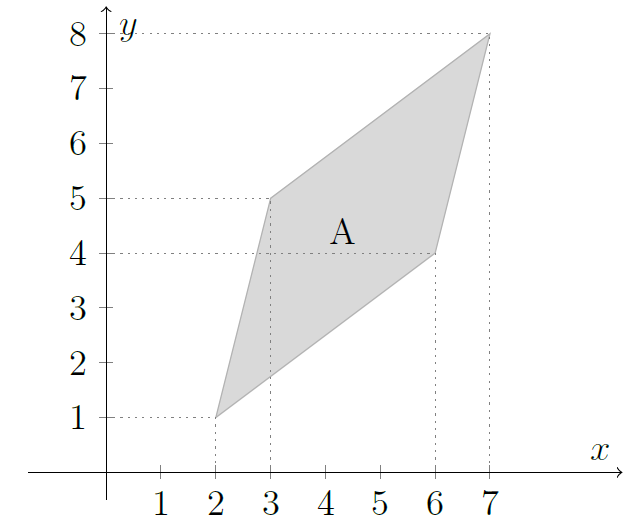
\includegraphics[width=0.7\textwidth]{pictures/aufgabe2_7}
\end{center}
Der Flächeninhalt $ A $ des Parallelogramms in der obigen Figur ist gleich
\renewcommand{\labelenumi}{(\alph{enumi})}
\begin{enumerate}
\item 
$ A = 10 $.
\item
$ A = 14 $.
\item
$ A = 5 \cdot  \sqrt{17} $.
\item
$ A = 16 $.
\item
$ A = 13 $.
\end{enumerate}
\ \\
\subsection*{\frage{8}{3}}
$ A $ sei eine $ (5 \times 5) $-Matrix gegeben durch
\begin{align*}
	A
	=
	\left[
	\textbf{a}_1,
	\textbf{a}_2,
	\textbf{a}_3,
	\textbf{a}_4,
	\textbf{a}_5
	\right].
\end{align*}
Sei 
\begin{align*}
	B =
	\left[
	\textbf{a}_1 - 3 \textbf{a}_2,
	\textbf{a}_2,
	\textbf{a}_3 + \textbf{a}_2 - \textbf{a}_5,
	-2 \textbf{a}_4,
	\textbf{a}_5
	\right].
\end{align*}
Dann gilt
\renewcommand{\labelenumi}{(\alph{enumi})}
\begin{enumerate}
	\item 
	$ \det(B) = -2 \det(A) $.
	\item
	$ \det(B) = \det(A) $.
	\item
	$ \det(B) = 6 \det(A) $.
	\item
	$ \det(B) = -\det(A) $.
	\item
	Es gibt im Allgemeinen keine Relation zwischen $ \det(A) $ und $ \det(B) $.
\end{enumerate}
\ \\
\subsection*{\frage{9}{2}}
Die Matrix $ A $ ist eine $ (7 \times 4) $-Matrix mit Rang $ 4 $.
Man bekommt die Matrix $ B $, indem man bei $ A $ die dritte Spalte streicht.\\
\\
Dann folgt:
\renewcommand{\labelenumi}{(\alph{enumi})}
\begin{enumerate}
	\item 
	$ \mathrm{rg}(B) = 4 $.
	\item
	$ \mathrm{rg}(B) = 3 $.
	
	\item
	$ \mathrm{rg}(B) < 3 $.
	
	\item
	Die Informationen reichen nicht aus, den Rang von $ B $ zu bestimmen.
\end{enumerate}
\ \\
\subsection*{\frage{10}{3}}
Welche der folgenden Aussagen ist \textit{falsch}?
\renewcommand{\labelenumi}{(\alph{enumi})}
\begin{enumerate}
	\item 
	Die Summe von zwei regulären Matrizen ist regulär
	\item
	Das Produkt von zwei singulären Matrizen ist singulär.
	
	\item
	Der Rang einer Matrix ist gleich dem Rang der Transponierten.
	\item
	Der Rang einer $ (n \times m) $-Matrix ist kleiner gleich $ n $, unabhängig davon, was $ m \in \mathbb{N} $ ist.
	\item 
	Die Summe zweier singulärer Matrizen kann regulär sein.
\end{enumerate}

\newpage
\section*{Aufgabe 3 (30 Punkte)}
\vspace{0.4cm}

\subsection*{\frage{1}{3}}
Die Funktion
\begin{align*}
	f(x,y) = 2^{xy}
\end{align*}
unter der Nebenbedingung
\begin{align*}
	\varphi(x,y)
	=
	x - 2 y - 2
	= 
	0
\end{align*}
hat
\renewcommand{\labelenumi}{(\alph{enumi})}
\begin{enumerate}
\item 
ein Minimum $ P = \left(1,-\frac{1}{2} \right) $.
\item
ein Maximum $ P = \left(1,-\frac{1}{2} \right) $.
\item
einen Sattelpunkt $ P = \left(1,-\frac{1}{2} \right) $.
\item 
Keine der obigen Aussagen ist richtig.
\end{enumerate}
\ \\
\subsection*{\frage{2}{4}}
Sei $ a \in \mathbb{R}_{++} $. Das bestimmte Integral
\begin{align*}
	\int_0^1
	\frac{1}{x^2} e^{\frac{a}{x}} dx
\end{align*}
ist gleich
\renewcommand{\labelenumi}{(\alph{enumi})}
\begin{enumerate}
	\item 
	$a e^{-a} $.
	\item
	$\frac{1}{a^2} e^{-a}$.
	\item
	$e^{-a} $.
	\item
	$\frac{1}{a} e^{-a}$.	
	\item
	Das Integral existiert nicht.
\end{enumerate}
\ \\
\subsection*{\frage{3}{4}}
Sei $ n \in \mathbb{N} $.
Das bestimmte Integral
\begin{align*}
	\int_0^1
	x(1-x)^n
	\ \td{x}
\end{align*}
ist gleich
\renewcommand{\labelenumi}{(\alph{enumi})}
\begin{enumerate}
	\item 
	$\frac{1}{n(n+1)}$.
	\item
	$\frac{n}{(n+1)(n+2)}$.
	\item
	$\frac{n}{n+1}$.
	\item
	$\frac{1}{n(n+2)}$.
	\item
	$\frac{1}{(n+1)(n+2)}$.	
\end{enumerate}
\ \\
\subsection*{\frage{4}{4}}
Gegeben ist die Matrix
\begin{align*}
	A
	=
	\begin{pmatrix}
		2 & a & -4 \\
		-1 & 3 & 4\\
		1 & -2 & -3
	\end{pmatrix}.
\end{align*}
Für welche Werte von $ a \in \mathbb{R} $ ist die Matrix $ A $
\textit{idempotent}, d.h., es gilt $ A^2 = A $?
\renewcommand{\labelenumi}{(\alph{enumi})}
\begin{enumerate}
\item 
$ a= 0 $.
\item 
$ a= -2 $.
\item
$ a= 2 $ oder $ a= -1 $.
\item
Es gibt kein $ a \in \mathbb{R} $, sodass $ A $ idempotent ist.
\item
$ A $ ist idempotent für jedes $ a \in \mathbb{R} $.
\end{enumerate}
\ \\
\subsection*{\frage{5}{4}}
Gegeben ist die Matrix
\begin{align*}
	A =
	\begin{pmatrix}
		1 & 0 & 2 & 3 \\
		2 & 1 & r & 7 \\
		3 & 2 & 4 &  s 
	\end{pmatrix}.
\end{align*}
Für welche Werte von $ r \in \mathbb{R} $ und $ s \in \mathbb{R} $ besitzt die Matrix $ A $ den Rang $ 2 $?
\renewcommand{\labelenumi}{(\alph{enumi})}
\begin{enumerate}
	\item 
	$ r = 10 $ und $ s = 2 $.
	\item 
	$ r =  2 $ und $ s = 10 $.
	\item
	$ r = 2 $ und $ s $ beliebig.
	\item
	$ r = 3 $ und $ s = 11 $.
	\item
	Die Matrix $ A $ hat für alle $ (r,s) \in \mathbb{R}^2 $ \textit{nicht} den Rang $ 2 $.
\end{enumerate}
\ \\
\newpage
\subsection*{\frage{6}{4}}
Gegeben ist die Matrix
\begin{align*}
	A =
	\begin{pmatrix}
		0 & 3 & 0 \\
		1 & 2 & 0 \\
		-5m & 5 & 4
	\end{pmatrix}
	, 
	\quad 
	\textrm{mit } m \in \mathbb{R}.
\end{align*}
Für den Eigenwert $ \lambda = -1 $ ist der Eigenraum $ W $ gegeben durch
\renewcommand{\labelenumi}{(\alph{enumi})}
\begin{enumerate}
	\item 
	$ W
	=
	\left\{
	\textbf{x} \in \mathbb{R}^3
	:
	\textbf{x}
	=
	s 
	\begin{pmatrix}
		3 \\ -1 \\ 1 - 3m
	\end{pmatrix},
	s \in \mathbb{R}
	\right\}
	 $
	.
	\item 
	$ W
	=
	\left\{
	\textbf{x} \in \mathbb{R}^3
	:
	\textbf{x}
	=
	s	 
	\begin{pmatrix}
		-3 \\ 1 \\ -1 - 3m
	\end{pmatrix},
	s \in \mathbb{R}
	\right\}
	$
	.
	\item
	$ W
	=
	\left\{
	\textbf{x} \in \mathbb{R}^3
	:
	\textbf{x}
	=
	s	 
	\begin{pmatrix}
		1 \\ -3 \\ 1 - 3m
	\end{pmatrix},
	s \in \mathbb{R}
	\right\}
	$
	.
	\item
	$ W
	=
	\left\{
	\textbf{x} \in \mathbb{R}^3
	:
	\textbf{x}
	=
	s	 
	\begin{pmatrix}
		3m \\ -1 \\ m-1
	\end{pmatrix},
	s \in \mathbb{R}
	\right\}
	$
	.
	\item
	$ \lambda = -1 $ ist kein Eigenwert von $ A $.
\end{enumerate}
\ \\
\subsection*{\frage{7}{3}}
Von der Lösung $ \{y_k\}_{k \in \mathbb{N}_0} $ der Differenzengleichung
\begin{align*}
	y_{k+1} = A y_k + B \quad (k = 0,1,2,...)
\end{align*}
sind die Werte
\begin{align*}
	y_0 = 2, y_1 = 1 \ \textrm{und} \ y_2 = 3
\end{align*}
bekannt.\\
\\
Bestimmen Sie $ A $ und $ B $.
\renewcommand{\labelenumi}{(\alph{enumi})}
\begin{enumerate}
\item
$ A=1 $ und $ B=2 $.
\item
$ A=2 $ und $ B=1 $.	
\item 
$ A=-1 $ und $ B=4 $.
\item
$ A=1 $ und $ B=2 $.
\item
$ A=-2 $ und $ B=5 $.
\end{enumerate}
\ \\
\subsection*{\frage{8}{4}}
Die allgemeine Lösung der  Differenzengleichung
\begin{align*}
(1+a) y_{k+1} + y_k -1 = 0
\quad (k = 0,1,2,...)
\end{align*}
mit $ a \in \mathbb{R} \setminus \{-1,-2\} $, ist genau dann monoton und konvergent, wenn
\renewcommand{\labelenumi}{(\alph{enumi})}
\begin{enumerate}
	\item
	$ a > 0 $.
	\item
	$ a >0 $ oder $ a < -1 $.	
	\item 
	$ -2 < a < 0 $.
	\item
	$ a < -2 $.
	\item 
	Die allgemeine Lösung $ \{y_k\}_{k \in \mathbb{N}_0} $ ist nie monoton und konvergent.
\end{enumerate}